\documentclass[../main.tex]{subfiles}

\begin{document}
\section{Sicurezza a Livello Trasporto: TLS}
\label{sec:tls}

\subsection{Introduzione a TLS}
\textbf{Transport Layer Security (TLS)} è una suite protocollare progettata per fornire servizi di sicurezza alle comunicazioni tra applicazioni. Si colloca tra il livello di trasporto (tipicamente TCP, ma anche UDP con DTLS) e il livello applicativo.

Gli obiettivi principali di TLS sono garantire:
\begin{itemize}
    \item \textbf{Autenticazione:} Verificare l'identità delle parti coinvolte (solitamente il server, opzionalmente il client).
    \item \textbf{Integrità:} Assicurare che i dati non vengano modificati durante la trasmissione.
    \item \textbf{Confidenzialità:} Proteggere i dati da intercettazioni, rendendoli illeggibili a terzi.
\end{itemize}
TLS stabilisce un canale di comunicazione sicuro e autenticato, utilizzando chiavi effimere derivate da credenziali crittografiche a lungo termine, come certificati X.509 (con le relative chiavi private) o Pre-Shared Keys (PSK).

\subsubsection{Breve Storia}
\begin{itemize}
    \item \textbf{SSLv2 (1995):} Sviluppato da Netscape per proteggere HTTP. Ora proibito per motivi di sicurezza.
    \item \textbf{SSLv3 (1997):} Correzione di bug di SSLv2, molto diffuso per anni. Deprecato nel 2015 perché insicuro.
    \item \textbf{TLSv1.0 (1999):} Standardizzazione IETF di SSLv3.
    \item \textbf{TLSv1.2 (2008):} Versione ampiamente utilizzata, con miglioramenti rispetto a v1.0. Introduce anche \textbf{DTLSv1.2 (2012)} per UDP.
\end{itemize}
Ci concentreremo su TLSv1.2 su TCP usando certificati X.509.

\subsection{Architettura Generale}
TLS è composto da diversi sotto-protocolli che lavorano insieme. L'architettura si appoggia al livello TCP/IP sottostante e interagisce con una libreria crittografica.

\begin{figure}[H]
  \centering
  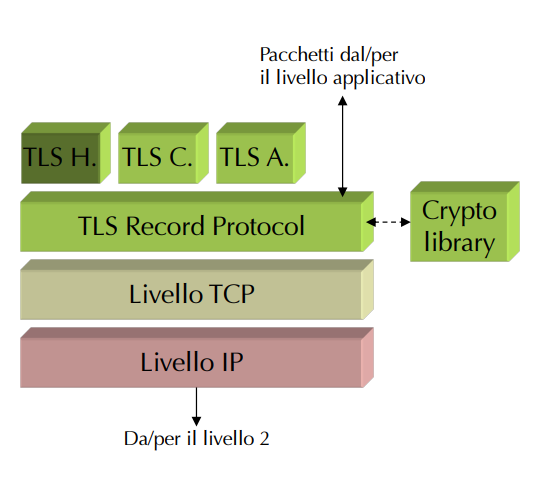
\includegraphics[width=0.6\textwidth]{TLSArch.png}
  \caption{Architettura Generale TLS}
  \label{fig:TLSArch}
\end{figure}

\subsubsection*{Descrizione Immagine: Architettura Generale TLS}
L'immagine mostra lo stack protocollare con TLS inserito tra le Applicazioni e il livello TCP.
\begin{itemize}
    \item In alto, i "Pacchetti dal/per il livello applicativo" entrano/escono dal livello TLS.
    \item Il cuore di TLS è il \textbf{TLS Record Protocol}. Questo protocollo riceve i dati dall'applicazione o dagli altri protocolli TLS (Handshake, ChangeCipherSpec, Alert), li frammenta, li comprime (opzionale), aggiunge un MAC, li cifra e li passa al "Livello TCP" sottostante. In ricezione, esegue le operazioni inverse.
    \item Sopra (o parallelamente) al Record Protocol ci sono i protocolli di controllo:
        \begin{itemize}
            \item \textbf{TLS H. (Handshake Protocol):} Negozia i parametri di sicurezza, autentica le parti e stabilisce le chiavi segrete.
            \item \textbf{TLS C. (Change Cipher Spec Protocol):} Segnala il passaggio dalla comunicazione non protetta a quella protetta con i parametri negoziati.
            \item \textbf{TLS A. (Alert Protocol):} Gestisce errori e notifiche.
        \end{itemize}
    \item A lato, una "Crypto library" fornisce le funzioni crittografiche (cifratura, hash, firme) utilizzate dai protocolli TLS.
    \item Sotto TLS ci sono i livelli standard "Livello TCP" e "Livello IP", che comunicano con il "Livello 2" (Data Link).
\end{itemize}

\subsubsection{TLS Record Protocol}
È il cavallo di battaglia di TLS. Una volta completato l'handshake, questo protocollo si occupa di:
\begin{itemize}
    \item Frammentare i dati applicativi in blocchi gestibili.
    \item Comprimere (opzionale).
    \item Aggiungere un MAC per l'integrità e l'autenticazione.
    \item Cifrare per la confidenzialità usando le chiavi derivate durante l'handshake.
    \item Passare i record cifrati a TCP.
\end{itemize}

\subsubsection{TLS Handshake Protocol}
È il protocollo più complesso, responsabile di:
\begin{itemize}
    \item Negoziare la versione del protocollo e la \textbf{cipher suite} (l'insieme di algoritmi da usare per scambio chiavi, cifratura simmetrica, MAC).
    \item Autenticare il server (tramite certificato) e opzionalmente il client.
    \item Stabilire le chiavi segrete condivise (\textbf{Master Secret}) usando meccanismi asimmetrici (es. RSA o Diffie-Hellman).
\end{itemize}
Poiché le operazioni asimmetriche sono costose, l'handshake stabilisce un \emph{Master Secret} per una \emph{sessione} TLS. Da questo Master Secret possono essere derivate in modo efficiente chiavi diverse per \emph{connessioni} multiple all'interno della stessa sessione.

\subsubsection{TLS Change Cipher Spec e Alert Protocol}
\begin{itemize}
    \item \textbf{Change Cipher Spec:} Un messaggio molto semplice (un solo byte) che indica che i messaggi successivi saranno protetti con i parametri appena negoziati.
    \item \textbf{Alert Protocol:} Usato per segnalare errori (es. certificato non valido, MAC errato, decifratura fallita) o altre condizioni (es. chiusura della connessione).
\end{itemize}

\subsection{TLS Handshake Protocol (Dettaglio)}
L'handshake di TLSv1.2 (con autenticazione basata su certificati RSA) prevede diversi passaggi tra Client (A, initiator) e Server (B, responder).

\begin{figure}[H]
  \centering
  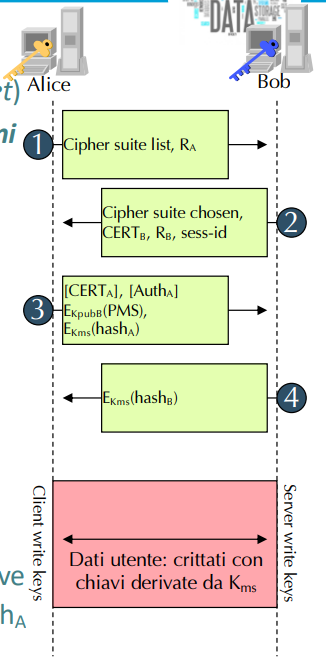
\includegraphics[width=0.7\textwidth]{TLSHandshake.png}
  \caption{Flusso Semplificato TLS Handshake}
  \label{fig:TLSHandshake}
\end{figure}

\subsubsection*{Descrizione Immagine: Flusso Semplificato TLS Handshake}
L'immagine mostra la sequenza di messaggi scambiati tra Alice (Client) e Bob (Server) durante l'handshake TLS per stabilire una sessione sicura.
\begin{enumerate}
    \item \textbf{Client Hello:} Alice $\to$ Bob.
        Contiene: la lista delle cipher suite supportate da Alice, un numero casuale $R_A$, e l'ID di sessione (se si vuole riprendere una sessione esistente).
    \item \textbf{Server Hello, Certificate, Server Hello Done:} Bob $\to$ Alice.
        Contiene: la cipher suite scelta dal server (tra quelle proposte da Alice), il certificato del server $CERT_B$ (contenente $K_{pubB}$), un numero casuale $R_B$, e l'ID di sessione. Il "Server Hello Done" (non mostrato esplicitamente) segnala la fine dei messaggi del server in questa fase.
    \item \textbf{Client Key Exchange, Change Cipher Spec, Encrypted Handshake Message:} Alice $\to$ Bob.
        \begin{itemize}
            \item \emph{(Opzionale) Certificate, Certificate Verify:} Se il server richiede l'autenticazione del client, Alice invia il suo certificato $CERT_A$ e una firma $Auth_A$ calcolata sui messaggi precedenti per provare il possesso della chiave privata $K_{privA}$.
            \item \emph{Client Key Exchange:} Alice genera un segreto pre-master (\textbf{PMS}, un altro numero casuale), lo cifra con la chiave pubblica del server ($K_{pubB}$ estratta da $CERT_B$), e lo invia: $E_{KpubB}(PMS)$.
            \item \emph{Change Cipher Spec:} Alice segnala che i messaggi successivi saranno cifrati.
            \item \emph{Encrypted Handshake Message (Finished):} Alice calcola il \textbf{Master Secret} ($K_{ms}$) a partire da PMS, $R_A$ e $R_B$. Calcola un hash di verifica ($hash_A$) su tutti i messaggi scambiati fino a quel punto, lo cifra con le chiavi derivate da $K_{ms}$ e lo invia: $E_{Kms}(hash_A)$.
        \end{itemize}
    \item \textbf{Change Cipher Spec, Encrypted Handshake Message:} Bob $\to$ Alice.
        \begin{itemize}
            \item Bob riceve il PMS cifrato, lo decifra usando la sua chiave privata $K_{privB}$. Ora anche Bob può calcolare lo stesso $K_{ms}$.
            \item \emph{Change Cipher Spec:} Bob segnala che i messaggi successivi saranno cifrati.
            \item \emph{Encrypted Handshake Message (Finished):} Bob calcola il suo hash di verifica ($hash_B$) su tutti i messaggi, lo cifra con le chiavi derivate da $K_{ms}$ e lo invia: $E_{Kms}(hash_B)$.
        \end{itemize}
    \item \textbf{Verifica e Sessione:} Alice decifra e verifica $hash_B$. Bob decifra e verifica $hash_A$. Se entrambi gli hash sono corretti, l'handshake è completato con successo. Alice e Bob condividono $K_{ms}$ e le chiavi da esso derivate (Client/Server write keys). La comunicazione applicativa può iniziare in modo sicuro.
\end{itemize}

\subsubsection{Autenticazione e Derivazione Chiavi}
\begin{itemize}
    \item \textbf{Autenticazione Server:} Alice autentica Bob verificando il suo certificato ($CERT_B$) tramite una CA fidata e verificando che Bob sia in grado di decifrare il PMS (possedendo $K_{privB}$) per calcolare correttamente l'hash finale $hash_B$.
    \item \textbf{Autenticazione Client (Opzionale):} Se richiesta, Bob autentica Alice verificando $CERT_A$ e la firma $Auth_A$.
    \item \textbf{Derivazione Chiavi:} Il \textbf{Pre-Master Secret (PMS)} è generato casualmente da Alice e inviato cifrato a Bob. Entrambi usano PMS e i numeri casuali scambiati ($R_A, R_B$) per calcolare indipendentemente lo stesso \textbf{Master Secret ($K_{ms}$)}. Da $K_{ms}$ vengono poi derivate le chiavi effettive per la cifratura e il MAC dei dati (Client write key, Server write key, ecc.).
\end{itemize}

\subsubsection{Note sull'Handshake}
\begin{itemize}
    \item \textbf{Perfect Forward Secrecy (PFS):} L'handshake descritto (basato su RSA Key Exchange) \textbf{non offre PFS}. Se un attaccante registra la sessione e successivamente ruba la chiave privata del server ($K_{privB}$), può decifrare il PMS e ricalcolare $K_{ms}$ e tutte le chiavi di sessione. Per ottenere PFS, è necessario usare cipher suite basate su \textbf{Diffie-Hellman Ephemeral (DHE o ECDHE)}, dove il PMS viene derivato tramite uno scambio DH invece che trasportato cifrato.
    \item \textbf{Catene di Certificati:} Durante l'handshake, il server (e opzionalmente il client) possono inviare non solo il proprio certificato, ma l'intera catena di certificati necessaria per la validazione fino a una Root CA fidata dal ricevente.
\end{itemize}

\subsection{Attacchi Noti a TLS/SSL}

\subsubsection{Heartbleed (2014)}
\begin{itemize}
    \item \textbf{Causa:} Bug nell'implementazione dell'estensione "Heartbeat" nella libreria OpenSSL (non un difetto del protocollo TLS in sé). L'estensione permetteva a un peer di inviare dati e chiedere all'altro di rimandarglieli indietro per verificare che la connessione fosse attiva.
    \item \textbf{Vulnerabilità:} Il richiedente specificava la lunghezza dei dati inviati e di quelli attesi in risposta. L'implementazione fallata non controllava che la lunghezza dichiarata corrispondesse a quella effettiva. Un attaccante poteva inviare pochi dati (es. 4 byte) dichiarando una lunghezza molto maggiore (es. 10000 byte).
    \item \textbf{Exploit:} Il server leggeva i 4 byte inviati e poi continuava a leggere dalla memoria adiacente al buffer per i successivi 9996 byte, inviando tutto all'attaccante.
    \item \textbf{Impatto:} Questa memoria "letta in eccesso" poteva contenere dati sensibili, inclusa la \textbf{chiave privata del server TLS}, password, cookie di sessione, ecc.. Con la chiave privata, un attaccante poteva decifrare traffico passato (se non si usava PFS) e impersonare il server.
    \item \textbf{Mitigazione:} Aggiornamento di OpenSSL e revoca/rinnovo dei certificati compromessi.
\end{itemize}
\begin{figure}[H]
  \centering
  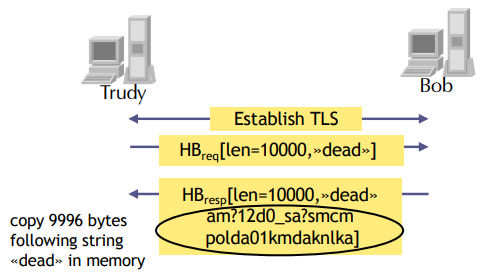
\includegraphics[width=0.8\textwidth]{Hb.png}
  \caption{Schema attacco Heartbleed}
  \label{fig:}
\end{figure}
\subsubsection{POODLE (2014)}
\begin{itemize}
    \item \textbf{Causa:} Vulnerabilità nel modo in cui SSLv3 gestisce il padding dei blocchi in modalità CBC (Cipher Block Chaining).
    \item \textbf{Vulnerabilità:} In SSLv3 CBC, il padding aggiunto per riempire l'ultimo blocco non è verificato correttamente dopo la decifratura. Un attaccante Man-in-the-Middle (MitM) può modificare l'ultimo blocco del ciphertext ($C_n$) e osservare se il server genera un errore di padding o meno.
    \item \textbf{Exploit (Padding Oracle):} Sostituendo $C_n$ con un blocco precedente $C_i$, l'attaccante può, byte per byte e con multiple richieste, dedurre il contenuto del blocco di plaintext $P_n$ (es. un cookie HTTP). L'attacco richiede prima un "downgrade" forzato della connessione a SSLv3, che l'attaccante può indurre intercettando i tentativi iniziali di connessione TLS e facendo credere a client e server che le versioni più recenti non siano supportate.
    \item \textbf{Impatto:} Permette a un attaccante MitM di decifrare parti del traffico protetto, come i cookie di autenticazione.
    \item \textbf{Mitigazione:} Disabilitare completamente SSLv3 su client e server.
\end{itemize}
\begin{figure}[H]
  \centering
  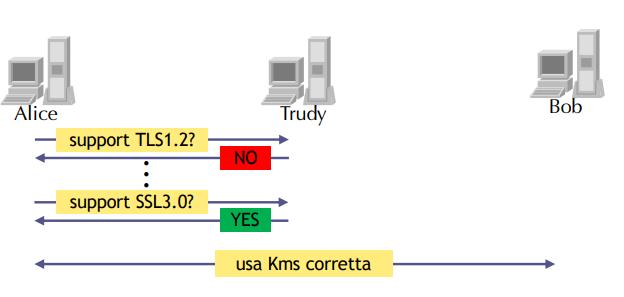
\includegraphics[width=0.8\textwidth]{POODLE.png}
  \caption{Schema attacco POODLE}
  \label{fig:}
\end{figure}
\subsubsection{Altri Attacchi (BEAST, CRIME, BREACH, DROWN)}
Sono stati scoperti altri attacchi che sfruttano debolezze in versioni precedenti di TLS/SSL o in funzionalità specifiche come la compressione o l'uso di CBC. Questi attacchi sottolineano l'importanza di:
\begin{itemize}
    \item Mantenere aggiornate le librerie crittografiche.
    \item Disabilitare versioni obsolete e insicure dei protocolli (SSLv2, SSLv3, TLSv1.0).
    \item Disabilitare funzionalità potenzialmente rischiose come la compressione TLS.
    \item Configurare correttamente i server per preferire cipher suite robuste che offrano PFS.
\end{itemize}

\end{document}
